\chapter{Planificación}
En este capítulo se va a realizar una planificación del TFG, en la que se
va a estimar el tiempo que se va a tardar en realizar cada tarea del proyecto
y el coste económico que supondría realizar el mismo.

\section{Metodología utilizada}
Para el desarrollo de la aplicación voy a enfocarlo con una metodología
tradicional, ya que es la que más cómoda me resulta y la que más se adapta
a este tipo de proyectos. Además, al ser un proyecto de una sola persona, no es
necesario utilizar una metodología ágil y desde mi punto de vista entorpecería
más el flujo de trabajo.

No es necesario utilizar una metodología ágil porque no hay un equipo de
desarrollo que coordinar en daily meetings, las tareas se realizarán de forma secuencial.
No hay un cliente o stakeholders que puedan cambiar los requisitos de forma
continua, por lo que no es necesario realizar entregas periódicas en sprints como
sí se hace en metodologías ágiles como Scrum. En nuestro caso no habrá feedback del
cliente ni reuniones de retroalimentación, sino que será una única persona la que
se encargará de realizar el control de calidad y verificar que se cumplan los
requisitos de la aplicación.

Para el control de calidad, pruebas y verificación de requisitos, se irá haciendo
de manera continua a medida que se vayan desarrollando las funcionalidades de la
aplicación.

\subsection{Seguimiento del proyecto}
Para el seguimiento del desarrollo de la aplicación se utilizará la herramienta
\textit{Trello} \cite{trello}, que permite crear tableros de kanban para oraganizar
las tareas pendientes de realizar, las que están en proceso y las que ya se han
realizado. Se puede ver el tablero kanban en la figura \ref{fig:trello}.

\begin{figure}[H]
  \centering
  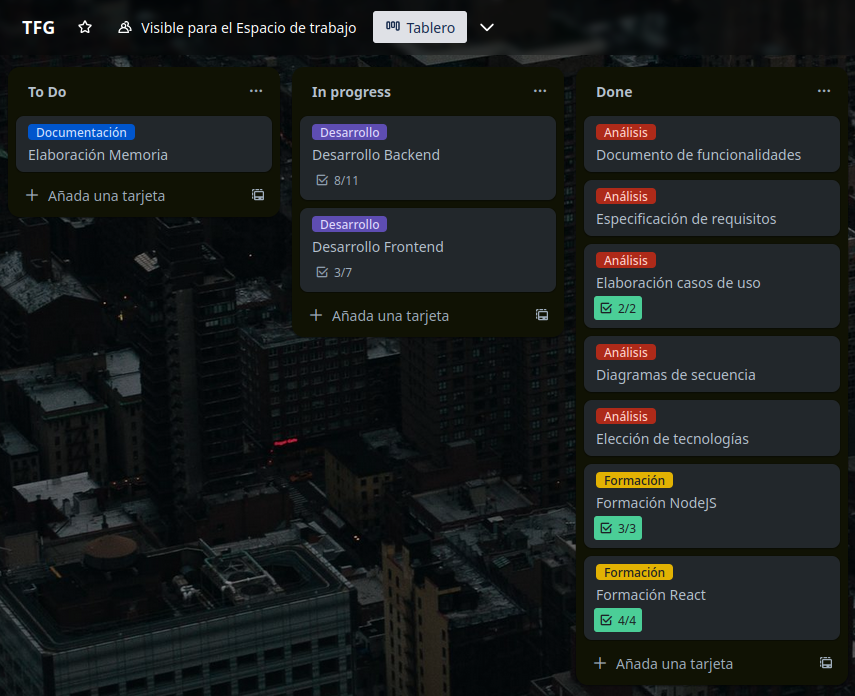
\includegraphics[width=1\textwidth]{trello}
  \caption{Tablero kanban de Trello}
  \label{fig:trello}
\end{figure}

\section{Control de versiones}
Para realizar un seguimiento del desarrollo de la aplicación se utilizará la
herramienta de control de versiones \textit{Git} \cite{git}, que permite llevar un
control de los cambios realizados en el código fuente de la aplicación. Además, estos
cambios se irán subiendo a la plataforma \textit{GitHub} \cite{github}.

\section{Temporización}
En esta sección se mostrará a través de un diagrama de Gantt la planificación
temporal del proyecto desglosado en tareas. Para ello se ha utilizado la
herramienta \textit{Lucidchart} \cite{lucidchart}.

\subsection{Diagrama de Gantt}
En la figura \ref{fig:gantt} se muestra el diagrama de Gantt con el desglose de las
tareas que se van a realizar, así como la duración de cada una de ellas en semanas.
Los colores diferencian las etapas del desarrollo del proyecto.
\begin{figure}[H]
  \centering
  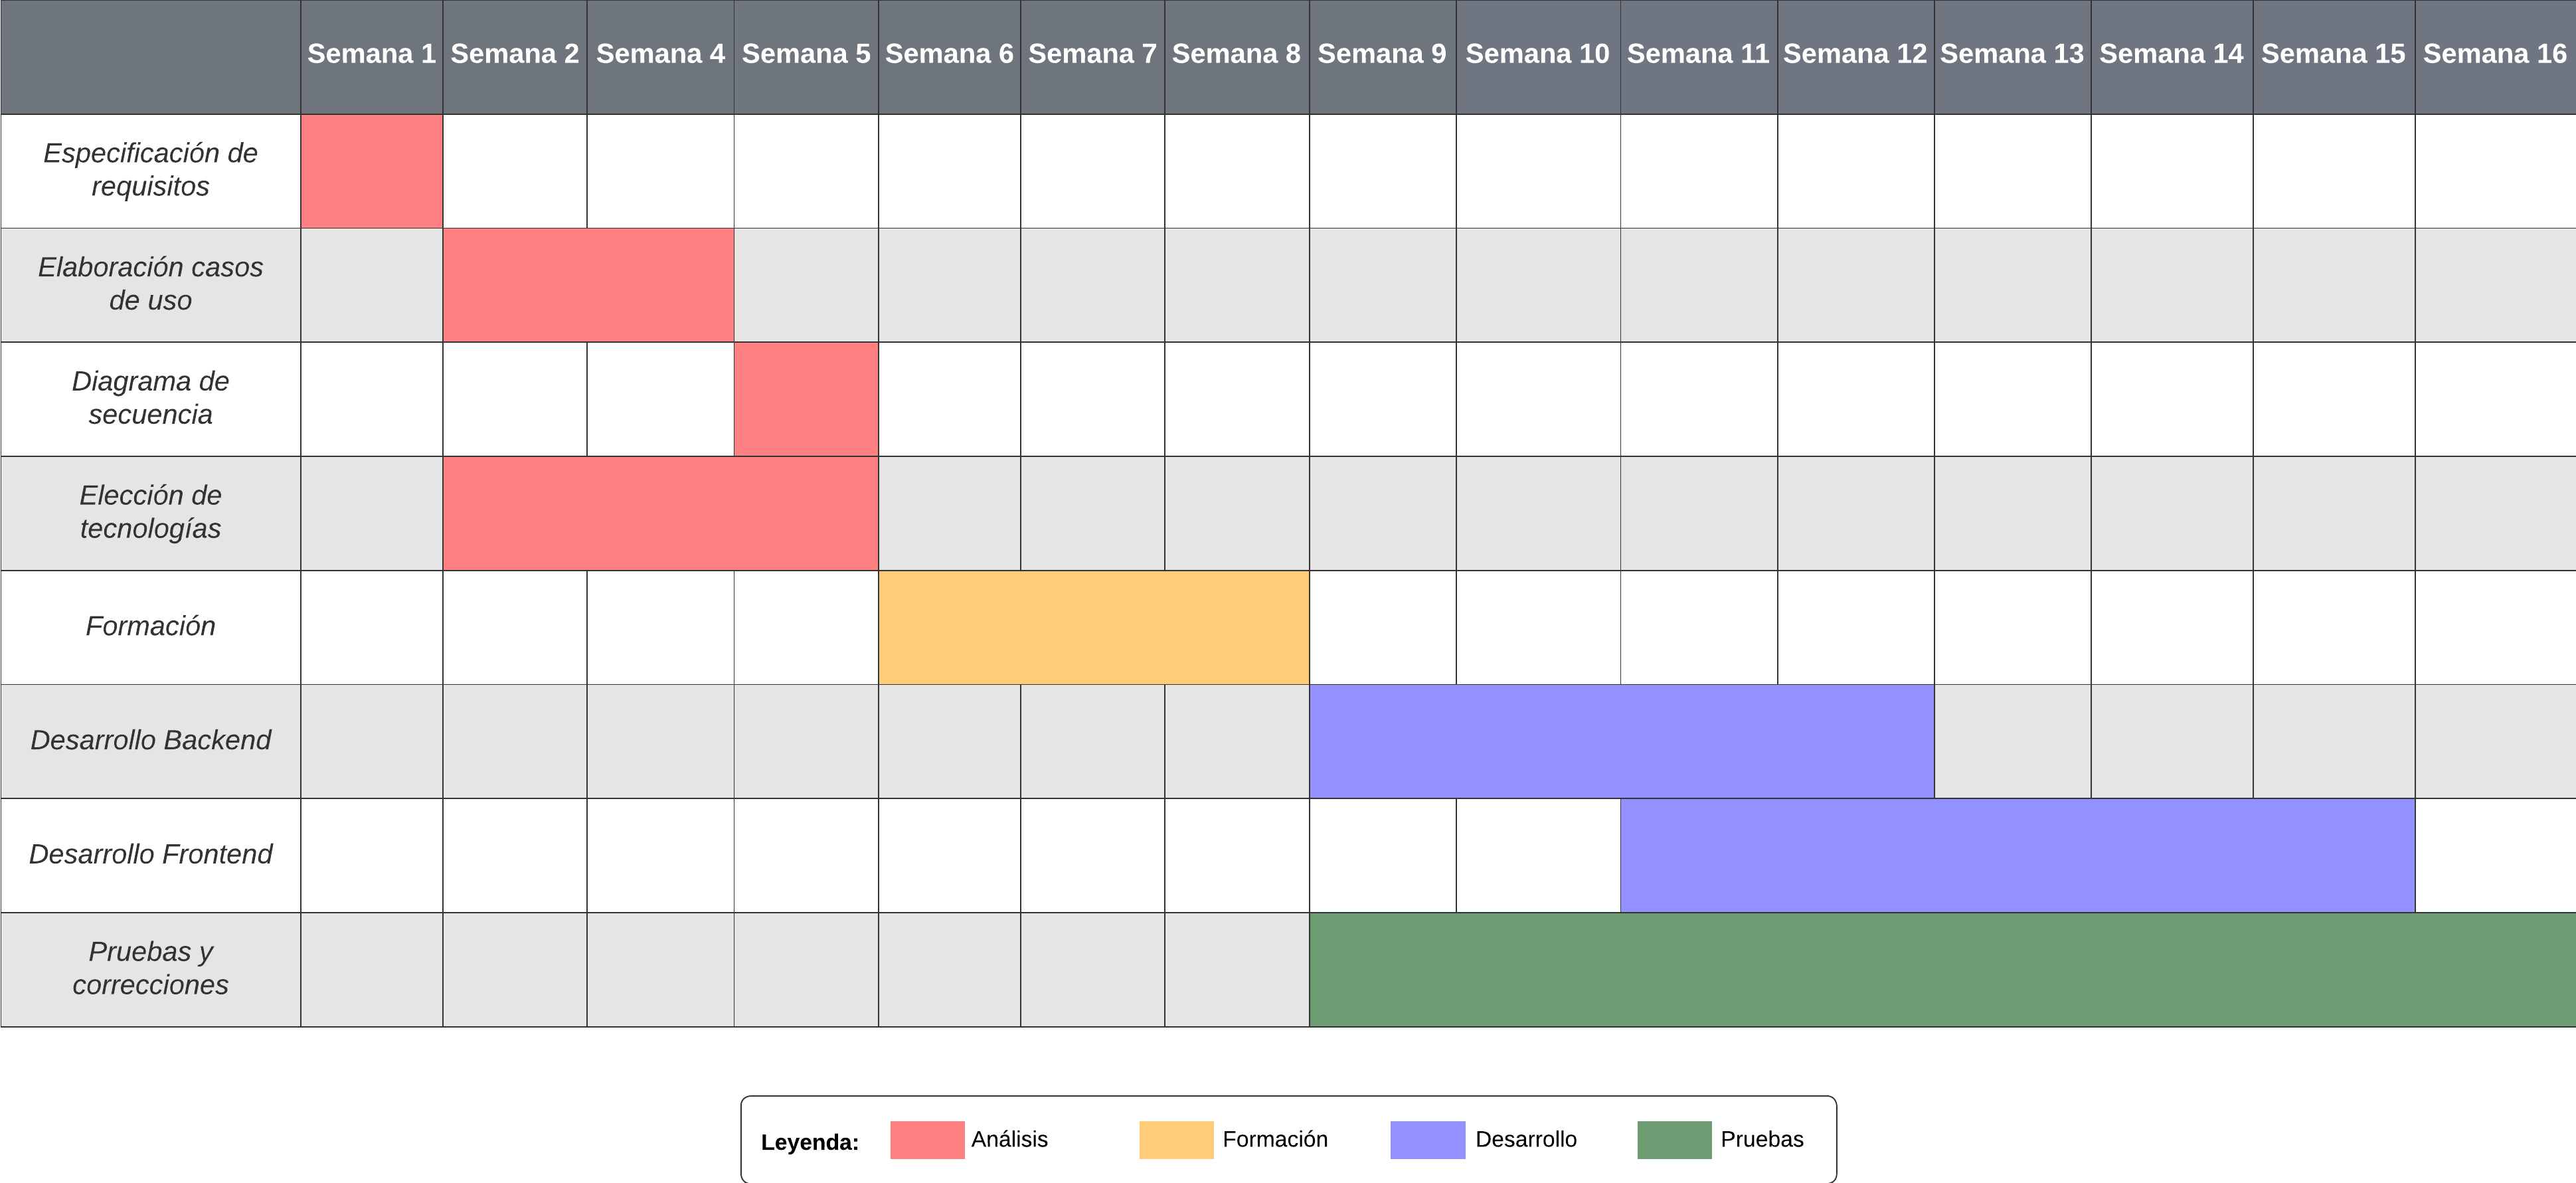
\includegraphics[width=1\textwidth]{gantt}
  \caption{Diagrama de Gantt}
  \label{fig:gantt}
\end{figure}

\section{Presupuesto}
